\documentclass[a4paper,12pt]{scrreprt}
    %% Used for changing geometry of the page
    %% Cover page text cannot overlay cover sketching/style 
    %% https://ctan.org/pkg/geometry?lang=en
\usepackage{geometry}
    %% Changes language of some packages protocols
    %% e.g., when captioning images: Figure 1. -> Figura 1.
    %% https://ctan.org/pkg/babel?lang=en
\usepackage[portuguese]{babel}
    %% Used for special fonts
    %% Cannot be compiled with pdflatex
    %% https://ctan.org/pkg/fontspec?lang=en
\usepackage{fontspec}
    %% Arial FONT
    \setmainfont{Arial}

    %% More colors and color options
    %% https://ctan.org/pkg/xcolor?lang=en
    %% https://ctan.org/pkg/colortbl?lang=en
\usepackage{xcolor,colortbl}
    %% More tabular options, like dashed/dotted lines
    %% https://ctan.org/pkg/arydshln?lang=en
\usepackage{arydshln}
    %% List of acronyms
    %% https://ctan.org/pkg/nomencl?lang=en
\usepackage[intoc]{nomencl}
    %% Must be called to init nomencl environment  
    \makenomenclature
    %% More images options/settings
    %% https://ctan.org/pkg/graphicx?lang=en
\usepackage{graphics}
    %% Defining subdirectories to image path enviornment
    %% \graphicspath{{sub1}{sub2}...{subN}}
    \graphicspath{{images}}
    
    %% used to handle cross-referencing commands in LaTeX to produce hypertext links in the document
    %% https://ctan.org/pkg/hyperref?lang=en
\usepackage{hyperref}
    %% math environments
    %% https://ctan.org/pkg/amsmath?lang=en

    %% settings
    \hypersetup{
        colorlinks,
        citecolor=black,
        filecolor=black,
        linkcolor=black,
        urlcolor=black
    }

\usepackage{amsmath}
    %% Defining backgrouns, used to make the cover
    %% https://ctan.org/pkg/background?lang=en
\usepackage[some]{background}
    %% Used to make drawings or complex graphics
    %% http://pgf.sourceforge.net/pgf_CVS.pdf
\usepackage{tikz}
    %% Tikz library to point operations ((x1,y1) + (x2,y2))
    \usetikzlibrary{calc}

%% Defining sfdefault font and default font for document
\renewcommand{\familydefault}{\sfdefault}


%% Costume made cover 
%% From there you can use \makecover command to build the cover
%% Blue cover color
\definecolor{titlepagecolor}{RGB}{54,95,145}

%==========================================================================
% COLORED BAR ON THE LEFT SIDE
%==========================================================================

\backgroundsetup{
    scale=1, 
    angle=0, 
    opacity=1,
    contents={
        \begin{tikzpicture}[remember picture,overlay]
            \path [fill=titlepagecolor] 
                (current page.north west) -- ($(current page.north west) + (5,0)$)
                -- ($(current page.south west) + (5,0)$)-- (current page.south west); 
            \node[color=white] at ($(current page.south west) + (3,4)$) {\bfseries {\fontsize{120}{60} \textsf{LI}}};
            \node[color=titlepagecolor] at ($(current page.south west) + (5.8,4)$) {\bfseries {\fontsize{120}{60} \textsf{4}}};
        \end{tikzpicture}
    }
}

%==========================================================================
% TITLE PAGE INFO
%==========================================================================

%% Changes values in this field to show information in the cover and back cover about your team/project


%% TITLE
\title{Sistema de Monitorização de Fogos}

%% AUTHORS
\author{
    Bruno Filipe de Sousa Dias A89583 \\
    Luís Enes Sousa A89597 \\
    Pedro Miguel de Soveral Pacheco Barbosa A89529
}

%% Date

\date{\today}

%% Course
\newcommand{\Course}{Mestrado Integrado em Engenharia Informática}

%% Department
\newcommand{\Department}{Escola de Engenharia}

%% UniName
\newcommand{\UniName}{Universidade do Minho}

%% UniPic
\newcommand{\UniPic}{
\includegraphics[scale=0.09]{images/uminho.png}}

%% University 
\newcommand{\University}{
    \begin{flushleft}
        \UniPic
    \end{flushleft}
    \textcolor{gray}{\small\textbf{\textsf{\UniName}}}\par
    \textcolor{gray!80!white}{\small{\textsf{\Department}}}\par
    \textcolor{gray!70!white}{\small{\textsf{\Course}}}
}

%% UC
\newcommand{\UC}{
    \begin{flushleft}
        \par\textcolor{titlepagecolor}{  \LARGE\textbf{\textsf{Unidade Curricular de \\ Laboratórios de Informática IV}}}
    \end{flushleft}
}

%% School Year
\newcommand{\SchoolYear}{
    \small{\textsf{Ano Letivo de 2020/2021}}}


%% Define new command to show title, author and date
\makeatletter
\let\Title\@title
\let\Author\@author
\let\Date\@date
\makeatother

%==========================================================================
% CLASSIFICATION SECTION 
%==========================================================================

%% School Year
\newcommand{\ReceptionDate}{}
%% Responsible
\newcommand{\Responsible}{}
%% Evaluation
\newcommand{\Evaluation}{}
%% Observations
\newcommand{\Observations}{}





%% MAKETEMPLATE
\newcommand{\makecover}{

%==========================================================================
% BEGIN COVER PAGE 
%==========================================================================

%% Removes page number on footer
\thispagestyle{empty}

%% No indentation 
\setlength{\parindent}{0em}

%% Put Background defined on \backgroundsetup, in this page
\BgThispage

%% Changing geometry to prevent overlay with text
%% At the end of back cover, geometry is default with \restoregeometry
\newgeometry{top=5cm,left=6cm,right=3cm,bottom=2cm}

%% builds university info defined previously
\University
\vspace{1cm}
%% builds curricular unity info defined previously
\UC
%% builds school year info defined previously
\SchoolYear

\vspace*{5cm}
%% bigger space (i think its the default one) between paragraphs 
\setlength{\parskip}{1em}

%% builds title info defined previously
\par\textbf{\textsf{\huge\Title}}
\vspace{1cm}
%% builds author(s) info defined previously
\par\Author

\vspace{0.5cm}

%% builds date info defined previously
\par\Date
\restoregeometry
\pagebreak

%==========================================================================
% END COVER PAGE 
%==========================================================================

%==========================================================================
% BEGIN BACK COVER PAGE 
%==========================================================================

%% Removes page number on footer
\thispagestyle{empty}

% Changing look of lines in tabular environment 
% Dashed -> dotted 
%% length of dashes
\setlength\dashlinedash{0.3pt}
%% space between dashes
\setlength\dashlinegap{1.5pt}
%% width of dashes
\setlength\arrayrulewidth{1.1pt}


%% This values can be changed in the preamble
\begin{flushright}
\begin{tabular}{ :p{4cm}:p{4cm}: } 
\hdashline
Data de Receção & \ReceptionDate \\ [2ex]
\hdashline
Responsável & \Responsible \\ [2ex]
\hdashline
Avalição & \Evaluation \\ [2ex]
\hdashline
Observações & \Observations \\ [7ex]
\hdashline
\end{tabular}
\end{flushright}


\vspace{10cm}
\begin{flushleft}

%% builds title info defined previously
\par\textbf{\textsf{\huge\Title}}
\vspace{1cm}
%% builds author info defined previously
\par\Author

\vspace{0.5cm}

%% builds date info defined previously
\par\Date
\end{flushleft}

\pagebreak
%==========================================================================
% END BACK COVER PAGE 
%==========================================================================
}


%% Command for using tabs
\newcommand{\tab}{
    \hspace{1cm}}

%==========================================================================
% DOCUMENT
%==========================================================================

\begin{document}

\pagenumbering{gobble}

% builds the cover
\makecover

%% smaller footer and header size
\newgeometry{top=3cm,left=3cm,right=3cm,bottom=4cm}

%==========================================================================
% BEGIN OPCIONAL DEDICATÓRIA
%==========================================================================
\iffalse
\clearpage
\begin{center}
    \thispagestyle{empty}
    \vspace*{\fill}

    \vspace*{\fill}
\end{center}
\clearpage
\fi
%==========================================================================
% END OPCIONAL DEDICATÓRIA
%==========================================================================


%==========================================================================
% BEGIN ABSTRACT PAGE
%==========================================================================



%% Abstract name: \Large font size, flushed left and paragraph skip before abstract content
\renewenvironment{abstract}
 {\par\noindent\textbf{\Large\abstractname}\par\bigskip}
 {}

\begin{flushleft}
\begin{abstract}
    \tab Este projeto surgiu com o intuito de auxiliar as pessoas na proteção do seu património, especialmente aquele situado nas zonas rurais, face aos incêndios florestais que tanto devastam a paisagem portuguesa. Desta forma, poderão ser evitados danos maiores e inesperados a terrenos ou habitações situadas em zonas de floresta.
    
    \tab Assim, será criada uma aplicação que alerta os seus utilizadores em caso de perigo iminente para as suas propriedades, permitindo-lhes atuar em tempo real face aos acontecimentos. Estes poderão, ainda, ter uma visão geral da situação, no território continental, em relação aos incêndios.

    \par \textbf{Área de Aplicação}: Minimização dos danos causados por incêndios florestais
    \par \textbf{Palavras-Chave}: Sistema de Monitorização, Incêndios, Engenharia de Software, Aplicações \textit{Web}, \textit{Microsoft}, \textbf{FIRESAFE}, Fundamentação, Especificação, Construção, Diagramas de \textit{Gantt}, \textit{UML}, Frontend, Backend.
\end{abstract}
\end{flushleft}


\pagebreak

%==========================================================================
% END ABSTRACT PAGE 
%==========================================================================

%==========================================================================
% BEGIN INDEXES PAGES
%==========================================================================

%% Changes table of content name
%% Portuguese babel default : "Conteúdo"
%% Personally I prefer "índice"
\renewcommand{\contentsname}{Índice}

\tableofcontents

\pagebreak

\listoffigures

\pagebreak

\listoftables

\pagebreak

%==========================================================================
% END INDEXES PAGES 
%==========================================================================


%==========================================================================
% BEGIN INTRODUCTION
%==========================================================================

%% Starting page numbering here
\pagenumbering{arabic}

\chapter{Introdução}
    \section{Contextualização}
        \tab O fogo e as maneiras de o obter e de o utilizar de maneira produtiva, foram cruciais para a sobrevivência da Humanidade e permitiram que o Homem iniciasse o  seu caminho em direção à civilização. Este pode surgir de modo indireto, através de catástrofes e eventos naturais, como relâmpagos, vulcões, (etc.), os quais foram os primeiros impactos dos homens primitivos com o fogo e dos quais retiraram as suas propriedades: a luz, o calor e sua capacidade de transmitir a chama a outros materiais. O fogo pode, também, ser adquirido através de métodos diretos e artificiais, como a fricção entre dois paus, o choque entre duas pedras e, até mesmo, com fósforos (como estamos habituados nos dias de hoje). Desconhece-se desde que altura se conseguiu obter fogo artificialmente, no entanto, existem vestígios e evidências que mostram que o fogo já era utilizado pelo Homem na Idade da Pedra, mais propriamente, no Paleolítico. Assim, percebemos que o fogo foi, e ainda é, fulcral para o ser humano continuar a existir. Ainda assim, nem sempre é usado da melhor forma e podemos, hoje, dizer que somos vítimas de algumas memórias melancólicas criadas pela tal força e exuberância que o fogo pode ter.
        
        \tab A 17 de Junho de 2017, no concelho de Pedrógão Grande, no distrito de Leiria, em Portugal, viveu-se uma grande tragédia, que percorreu os corações de milhões de Portugueses e as bocas de milhões de cidadãos do mundo. Uma tragédia que levou consigo a vida de 66 pessoas, deixando mais de 200 feridas e destruindo cerca de 500 habitações. O fogo destruiu ainda 53 mil hectares de território, 20 mil dos quais de floresta, durante 7 longos dias \cite{incendio_pedrogao}.
        
        \tab É então nesta altura, que, em Portugal, começa a aparecer uma melhoria das medidas de prevenção contra os fogos e uma melhoria e criação de aplicações de controlo e de alerta para possíveis incêndios, por parte de várias empresas. Consigo, nasce a ideia da \textbf{FIRESAFE}, que é uma aplicação de desenvolvimento de software orientada à monitorização de incêndios e de possíveis riscos dos mesmos, de modo a aumentar a segurança de todos os cidadãos e de intensificar a prevenção de possíveis grandes catástrofes.
\clearpage
    \section{Apresentação do Caso de Estudo}
        \tab A \textbf{FIRESAFE} é uma aplicação orientada à monitorização de incêndios e de possíveis riscos dos mesmos acontecerem. Assim, esta irá permitir às pessoas serem devidamente avisadas e poderem tomar as suas precauções face a possíveis desastres.
        
        \tab A implementação deste sistema será feita para a utilização em clientes universais (\textit{Web browsers}) e, deste modo, os utilizadores apenas irão necessitar aceder ao endereço da aplicação através de qualquer browser, disponível no seu computador, smartphone, etc. Posto isto, o utilizador da aplicação é então munido com 2 opções: efetuar o login (ou o registo caso nunca se tenha registado) ou utilizar a aplicação sem efetuar o login. No entanto, caso não seja efetuado o login, o utilizador deixa de ser dotado de algumas funcionalidades que irão ser abordadas seguidamente.
        
        \tab Em qualquer um dos tipos de uso o utilizador possui um conjunto de funcionalidades comum a ambos. Neste momento, podemos consultar um mapa de Portugal Continental onde podemos ver várias informações. Neste mapa, podemos ver quais os incêndios que se encontram nos vários estados (no seu início, a decorrer, em resolução ou até dados como concluídos) em Portugal. Em cada incêndio podemos ainda ver informações climatéricas da zona/região do mesmo e dados relativos ao número de humanos, número de veículos terrestres e número de veículos aéreos em intervenção. Podemos, ainda, obter informações relativas às horas dos respectivos estados do incêndio, bem como de possíveis alturas de alerta.
        
        \tab Além destas funcionalidades, o utilizador pode fazer o seu registo na aplicação, tal como mencionado anteriormente. Neste registo, o utilizador fornece os seus dados e algumas informações pessoais tais como: o nome, um username, o e-mail, um número de telemóvel (opcional), a sua data de nascimento, uma password e outros possíveis dados individuais. Encontrando-se registado no sistema, o utilizador pode, então, realizar o seu login. Efetuado o login, o utilizador tem a possibilidade de adicionar localizações favoritas. Adicionando estas localizações, o utilizador irá ser notificado caso exista um incêndio nas proximidades ou caso o risco de incêndio nos próximos dias seja elevado.

    \section{Motivação e Objectivos}

        \tab Portugal é um país muito fustigado por incêndios florestais, especialmente durante o verão. Em 2019, registaram-se 10832 fogos, totalizando 42084 ha de área ardida \cite{relatorio_fogos_2019}. Embora tenha havido melhorias nos últimos anos, os números ainda são algo preocupantes.
        
        \tab Sendo assim, achamos importante desenvolver uma aplicação capaz de alertar os seus utilizadores da ocorrência de incêndios nas proximidades de localizações do seu interesse, de forma a evitar catástrofes maiores. Já é possível receber alertas através de SMS, no entanto, apenas são enviados quando sucedem incêndios de nível bastante elevado. Para além disso, não são enviados alertas customizados consoante as preferências do utilizador, nem é enviada nenhuma informação quando acontecem pequenos incêndios. Estes pequenos incêndios podem ser menosprezados por este sistema de alertas, no entanto, eles podem ser fatais para habitações, terrenos rurais ou, até mesmo, pelo facto de aumentarem o risco de acidentes face a possíveis rotas que possamos ter no dia a dia. O facto de não termos encontrado nenhuma aplicação com esta finalidade também influenciou a nossa decisão, aspirando a resolução deste problema.
        
        \tab Pretendemos, então, resolver um problema há muito conhecido, mas ainda com poucas soluções. A sua primazia será a customização pessoal, para que cada um possa usufruir da melhor forma possível da aplicação. Alargamos o envio de alertas para todo o tipo de incêndios (mesmo os mais insignificantes) para a maior segurança de todos, ao contrário do que já encontramos hoje, que, ou possuímos poucos alertas, recebendo apenas os que estão relacionados com os casos mais intensos, ou então recebemos uma quantidade de informação em demasia e a informação que nos é mais relevante é perdida. Esperamos poder aumentar a segurança das pessoas num dos aspetos da sua vida, tendo como objetivo deliciar as pessoas com o melhor serviço disponível. Dada a abundância destes acontecimentos no verão, detemos, também, como meta a finalização da construção deste serviço até à data estipulada, fazendo com que a aplicação esteja já disponível no decorrer do próximo que se avizinha.

    \section{Estrutura do Relatório}
        \tab No presente relatório demonstramos a primeira etapa da construção do serviço e da aplicação \textbf{FIRESAFE}, que passa pelo Domínio da Engenharia de Software, com particular ênfase no desenvolvimento de aplicações. A construção do software em questão é orientado, principalmente, ao desenvolvimento de um Sistema de Monitorização de Eventos.
        
        \tab A primeira fase do projeto é denominada de Fundamentação. Nesta etapa são tidos como principais objetivos fundamentar, projetar e gerir o desenvolvimento de um sistema de software.
        
        \tab Dessa forma, começamos por expor uma explicação, exibindo uma contextualização sobre o tema. Após ser mostrado o contexto em que estaremos a trabalhar, são apresentadas todas as motivações para a construção do projeto em questão, bem como a implementação que pretendemos engenhar. Além disso, são ainda expressos todos os objetivos que pretendemos alcançar, tanto a nível de realização da empresa, como da satisfação do utilizador comum.
        
        \tab Seguidamente, são identificadas as justificações, a viabilidade e ainda a utilidade do sistema, onde é explicado, de forma mais prática, as vantagens da utilização e da construção deste sistema, bem como a praticabilidade e a exequibilidade do mesmo.
        
        \tab Após isso, é estabelecida a Identidade do Projeto, onde são identificadas várias características e informações sobre a aplicação. Nestas informações podem estar referências ao nome da empresa, faixa etária de utilização, uma breve descrição, entre outras.
        
        \tab Posto isto, é necessário perceber quais os recursos que serão necessários para podermos efetuar a construção deste sistema e a realização deste projeto com sucesso. Aqui, é descrita a forma como iremos obter todos os dados necessários.

        \tab Expostos os tipos de dados necessários, chega, então, o momento de explicar a forma como esses dados são utilizados, realizando uma Maqueta do Sistema onde são evidenciadas as funcionalidades da aplicação e a forma como estas podem ser feitas.
        
        \tab Como em todos os bons projetos, é preciso perceber que medidas implementar para que este seja realizado com êxito. Assim, são apresentadas medidas de sucesso.
        
        \tab Por fim, é preciso fazer uma gestão de toda esta construção. Esta é uma etapa crucial no âmbito da Engenharia de Software, já que é neste momento que se pode fazer a melhor gestão e o melhor acompanhamento de um projeto de Desenvolvimento de Software. É, então, nesta fase, apresentado um plano de desenvolvimento, onde são divididas as tarefas pelos vários elementos do grupo, de modo a toda a equipa conseguir produzir o melhor resultado possível, sem causar fadiga desnecessária de certos elementos ou acontecerem acidentes com datas de entrega e material atrasado.
        
        \tab Posteriormente a esta fase, serão ainda realizadas mais duas fases. É realizada uma segunda fase denominada Especificação, onde será feita uma análise e serão especificados, de forma completa, todos os requisitos operacionais e funcionais de um sistema de software. Por fim, será realizada uma terceira fase, denominada de Construção, onde iremos ingressar no processo de desenvolver, validar, documentar e instalar sistemas de software.
        
    \section{Justificação do Sistema}
        \tab Os incêndios são das catástrofes naturais mais graves em Portugal, tanto pela elevada frequência com que acontecem, como pelos seus efeitos de destruição e grandes prejuízos económicos e ambientais que trazem. Todos os anos, em Portugal, são registados milhares de fogos, que trazem consequências, muitas vezes fatais, para as famílias e para a sociedade portuguesa. Durante o verão, principalmente, muitas habitações e terrenos são destruídos à custa dos incêndios florestais. Muitas vezes, os donos dessas propriedades podem até só receber essa informação vários dias depois, quando já nada pode ser feito para evitar os danos. Contudo, e apesar de não ser possível evitar totalmente uma catástrofe natural, no caso de haver um melhor controlo destes desastres a sociedade poderia, muitas vezes, salvar os seus bens, retirar os seus animais de casa quando o fogo estivesse próximo, ou até mesmo salvar um idoso que, naturalmente, teria dificuldades em fazê-lo sozinho. Assim, surgiu a ideia da nossa aplicação, que poderá ser útil na prevenção desses casos, pois avisa, em tempo real, potenciais ameaças.

    \section{Utilidade do Sistema}
        \tab O nosso sistema pretende ser uma ajuda na prevenção de catástrofes relacionadas com os incêndios florestais. Como referido anteriormente, a aplicação será capaz de detetar incêndios nas proximidades de locais à escolha do utilizador. O utilizador poderá, ainda, ser notificado caso seja detetado risco elevado de incêndio numa dessas localizações. Uma vez que os dados são atualizados em tempo real, o utilizador pode reagir imediatamente, podendo evitar grandes catástrofes. Noutro ponto de vista, um utilizador pode, por exemplo, querer passar uns dias num belo acampamento rodeado de densa vegetação. Neste caso, o utilizador pode verificar, atempadamente, antes de sequer se deslocar até ao local, se existem incêndios nessa zona ou nas suas imediações, fazendo, depois,  a escolha de ingressar para a sua viagem ou não. Pode ainda visualizar o tipo de risco de incêndios que a zona pretendida terá nos próximos dias. Tudo isto é disponibilizado de forma gratuita, sem quaisquer custos ou obrigações, facilitando ainda mais o processo de uso da aplicação.

    \section{Viabilidade do Sistema}
        \tab Nos dias de hoje, a tecnologia encontra-se bastante avançada e, por isso, tudo aquilo que queremos está muitas das vezes à distância de um clique. Esta aplicação não será exceção. Tal como referido anteriormente, os incêndios florestais trazem molestos problemas à sociedade e é necessária uma solução para tal. A nossa aplicação tem como intuito travar muitos desses danos, com uma ideia inovadora e ainda não implementada, o que nos faz acreditar que será uma aplicação com bastante procura. Podemos usufruir deste serviço através de qualquer browser, em qualquer tipo de dispositivo. No entanto, para um maior proveito, o utilizador deve criar uma conta, registando-se e inserindo dados pessoais que qualquer cidadão no mundo atual possui: um e-mail e um número de telemóvel (opcional), entre outros dados menos fulcrais. Após isso, poderá identificar quais as zonas/localizações a monitorizar. Assim, aquando de um incêndio, o utilizador poderá receber notificações no ecrã (caso esteja com a aplicação aberta) ou por e-mail. Deste modo, podemos estar em qualquer lugar com acesso à Internet que iremos receber um e-mail ou os devidos alertas, consoante as localizações que indicamos, de modo a podermos reagir da forma mais rápida possível. 

    \section{Estabelecimento da Identidade do Projeto}
        \begin{itemize}
            \item {\large \textbf{Nome:}} \textbf{FIRESAFE}
            \item {\large \textbf{Categoria:}} Sistema de Monitorização
            \item {\large \textbf{Idioma:}} Português
            \item {\large \textbf{Faixa Etária:}} Todas as idades
            \item {\large \textbf{Descrição:}} O sistema de monitorização é facilmente acessível através de um Web Browser, sendo que qualquer utilizador consegue ter acesso à aplicação através de qualquer aplicativo que lhes permita acesso a um browser. Tendo feito o acesso é apresentado ao utilizador um mapa de Portugal Continental, interativo, onde este conseguirá observar todos os incêndios ocorridos nas últimas 24h, quer estejam estes ativos, a ser combatidos ou extintos. O utilizador consegue, ainda, saber se determinada área corre risco de incêndio para o próprio dia de visualização ou para o dia seguinte e ainda selecionar um incêndio para obter informações sobre o mesmo. Se este decidir efetuar um registo (ou dar login caso já se tenha registado), consegue, ainda, escolher uma localização para monitorizar com o intuito de receber um alerta caso esta tenha um incêndio ativo nas proximidades ou seja previsto risco elevado de incêndio nessa zona.
            \item {\large \textbf{Empresa:}} NTH371
            \item {\large \textbf{Criadores:}} Bruno Dias, Luís Sousa e Pedro Barbosa
            \item {\large \textbf{Logotipo:}} 
                \begin{figure}[hbt!]
                    \centering
                    \frame{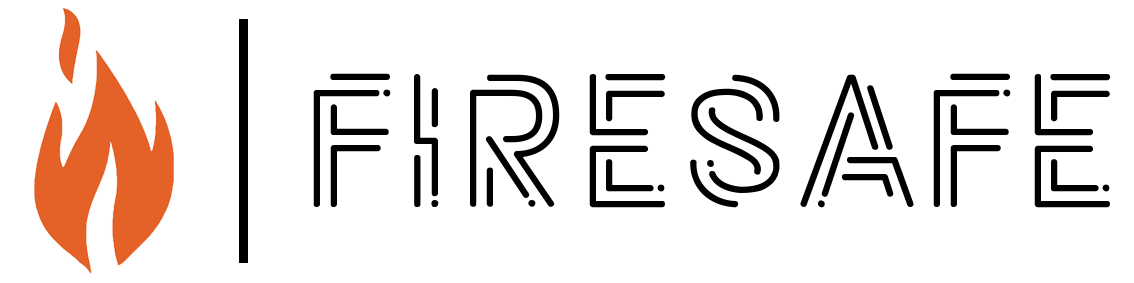
\includegraphics[width=.7\textwidth]{images/Fase1/logoFIRESAFE.png}}
                    \caption{Logotipo}
                \end{figure}
        \end{itemize}
        
        \tab Tendo em conta esta ficha de projeto, a nossa aplicação estará disponível e poderá ser acedida por qualquer pessoa desde que esta tenha acesso a um browser. A nossa empresa, inicialmente, tentará contactar e implementar a aplicação nos diversos corpos de bombeiros do país, sejam estes municipais ou voluntários, pois percebemos que são o principal foco de combate ao problema que tentamos resolver e que, juntamente com a correta utilização da \textbf{FIRESAFE}, irão lutar contra esse mesmo problema que Portugal enfrenta.

    \section{Identificação dos recursos necessários}
        \tab Sendo que a empresa NTH371 teve a ideia de construir uma aplicação para a minimização dos danos causados por incêndios florestais, é então necessário reunir um conjunto de recursos que serão necessários para a concessão da mesma. Dessa forma, e como primeiro instinto, os seus criadores foram em busca de informação através das pessoas que mais sofrem com tais catástrofes, e com as quais lidam todos os dias, ou seja, os bombeiros.

        \tab Desta maneira chegou-se a alguns aspetos que seriam cruciais contemplarmos na nossa aplicação. Os dados tinham de ser atualizados o mais rapidamente possível, uma vez que o fogo se pode espalhar de forma muito rápida e é necessário reagir sempre da forma mais breve possível. Outro aspeto que seria bastante importante é possuir grande informação acerca do incêndio e do local (se se está a alastrar, se está a ser apagado, se está resolvido, se está apenas a iniciar-se e também o seu risco, de baixo a muito elevado). Além disso, é ainda importante o aspeto de poder receber notificações em qualquer lugar, a qualquer instante, de forma imediata.
        
        \tab Posto isto, é necessário escolher as ferramentas a utilizar de maneira a  obtermos o melhor sucesso na construção do sistema. Para a concessão de relatórios e de futuras apresentações, optamos por escolher produtos provenientes do \textit{Microsoft Office}. Como sustento à criação e gestão de futuras bases de dados utilizadas, iremos operar com o sistema da \textit{Microsoft SQL Server}. Seguindo o que vemos como regra neste projeto, iremos também utilizar a \textit{Microsoft .NET C\#} como plataforma de desenvolvimento. Para editor de texto, a equipa decidiu usufruir do \textit{Microsoft Visual Studio} por acharmos ser o mais compatível com a área e o tipo de software com que iremos trabalhar. Ainda é, contudo, necessária uma ferramenta fulcral na conceção desta aplicação. Esta ferramenta será uma \textit{API} que nos permitirá acessar dados a uma certa fonte de informações e de facto dar asas à parte da Monitorização de Eventos. De momento não vemos um uso necessário para a concessão de certas funcionalidades através de comandos de voz, no entanto, se utilizarmos essa função futuramente, pretendemos utilizar também uma \textit{API} da \textit{Microsoft}, denominada \textit{Microsoft Speech Platform}.

    \section{Maqueta do sistema}
        \tab A implementação deste sistema será feita para a utilização em clientes universais (\textit{Web browsers}) e, deste modo, os utilizadores apenas irão necessitar aceder ao endereço da aplicação através de qualquer browser, disponível no seu computador, smartphone, etc. Posto isto, é apresentado um mapa de Portugal Continental interativo, onde se podem ver os incêndios ocorridos nesse território nas últimas 24 horas, estejam eles ativos, em resolução ou extintos. O utilizador pode ainda verificar o risco de incêndio para o próprio dia ou para o dia seguinte consoante cada localização, mais propriamente, por concelho. Dentro de cada incêndio podemos ainda visualizar informações relativas ao mesmo e ao seu combate, ou seja, temperaturas, número de meios utilizados, onde se inserem meios humanos, terrestres e aéreos, entre outros dados.
   
        \tab Caso o utilizador se autentique na aplicação, através de um registo (ou login, caso se tenha registado anteriormente), este pode definir uma localização a monitorizar, recebendo um aviso caso ocorra um incêndio nas proximidades ou caso esteja previsto risco elevado de incêndio. Pode, ainda, eliminar uma localização previamente selecionada. Cada utilizador pode ainda mudar de número de telemóvel, e-mail e outras informações pessoais do seu perfil. Posto isto, o utilizador pode, também, definir o tipo de notificações que pretende receber, ou seja, pode escolher notificações no ecrã, por e-mail ou até mesmo um conjunto das várias opções mencionadas.
        
        \tab Em baixo, apresentamos uns esboços feitos através do Software \textit{Justinmind}, de como estamos a pensar organizar a nossa aplicação, nomeadamente, a página inicial com o mapa interativo de Portugal Continental e um pequeno menu com as informações relativas a um dado incêndio.
        
        \vspace{0.6cm}
        
        \begin{figure}[hbt!]
            \centering
            \frame{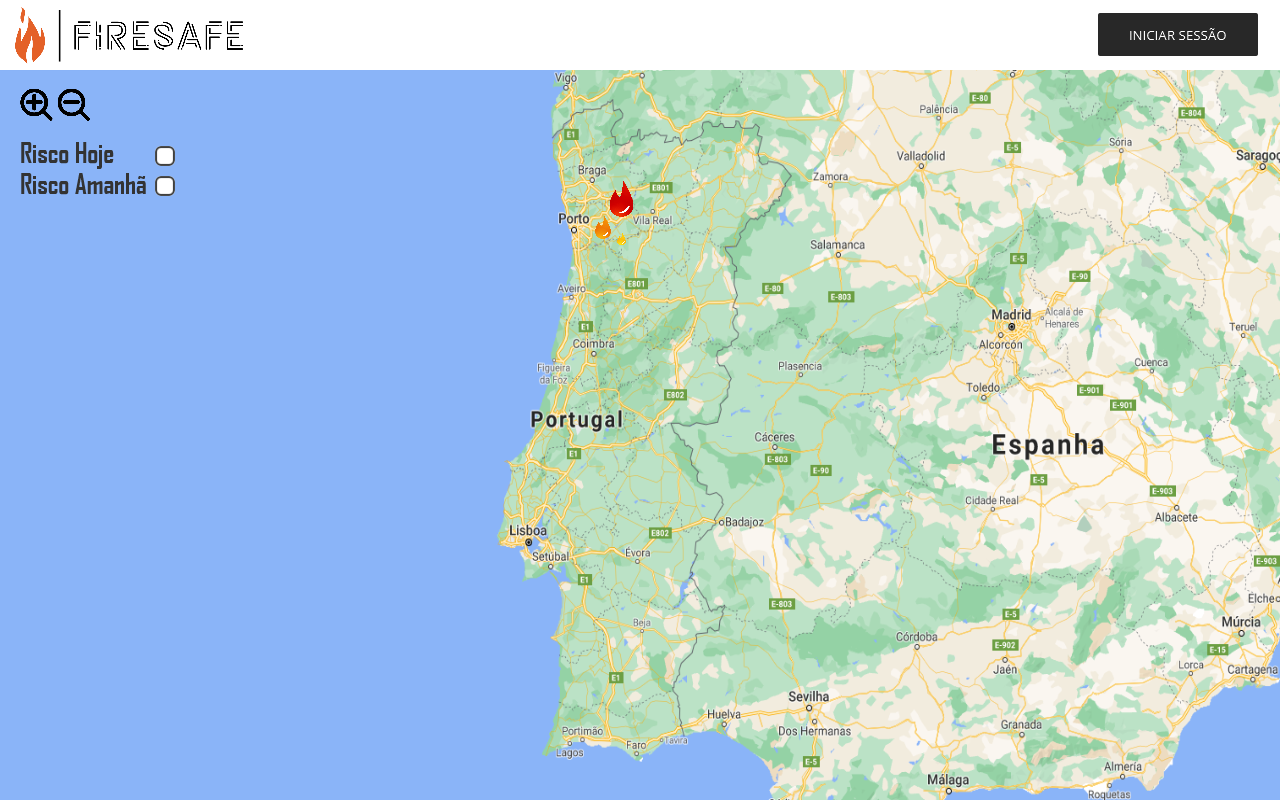
\includegraphics[width=.8\textwidth]{images/Fase1/pagina_inicial.png}}
            \caption{Página inicial}
        \end{figure}
        
        \begin{figure}[hbt!]
            \centering
            \frame{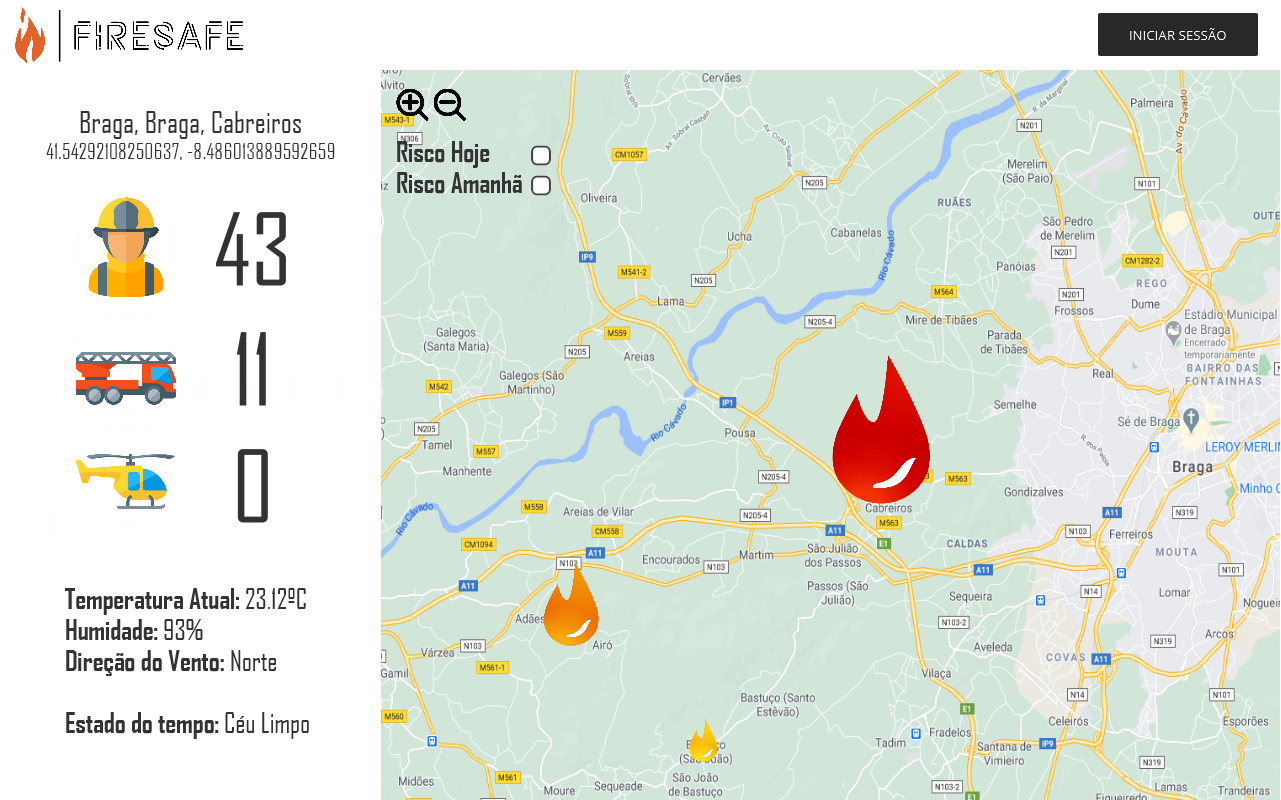
\includegraphics[width=.8\textwidth]{images/Fase1/menu_incendio.png}}
            \caption{Menu relativo a um incêndio}
        \end{figure}

    \section{Definição de um conjunto de medidas de sucesso}
        \tab Nos dias que correm, definir um conjunto de medidas de sucesso de um determinado projeto é uma das etapas consideradas fulcrais no desenvolvimento de software nas empresas. Uma avaliação global de tudo aquilo que possa ter corrido mal durante o processo de desenvolvimento torna possível a minimização de erros em futuros projetos e também aumenta as chances de sucesso.
        
        \tab Desta forma, para que o nosso projeto alcance o sucesso desejado, definimos as seguintes medidas. Relativamente ao planeamento, dividimos todos os processos e etapas do trabalho de forma a garantir o cumprimento de todos os prazos de entrega existentes. No que se refere à organização do grupo, confiamos o projeto a uma pessoa que achamos que reúne todas as qualidades necessárias para chefiar a equipa mantendo a harmonia e um bom ritmo de trabalho de todos os elementos, assim como garantir que todos trabalhamos para um determinado objetivo, sendo este comum a todos. No que diz respeito ao método utilizado para garantirmos o reconhecimento e utilização da nossa aplicação, o nosso grupo acredita piamente que é apostando na publicidade que iremos encontrar o nosso maior sucesso. Desta forma, iremos controlar o nosso orçamento restante e gastá-lo a publicitar a nossa aplicação através dos meios que nos forem disponibilizados. Também nos comprometemos a sensibilizar a população portuguesa para o problema dos incêndios, sobre o qual a nossa aplicação incide e pretende minimizar os problemas a este acarretados, e a tentar alcançar os diferentes corpos de bombeiros do país (segundo a \textit{PORDATA}, rondavam um total de 465 no ano de 2019 \cite{corpos_bombeiros}) de forma a tentar uniformizar a utilização da nossa aplicação pelos mesmo, o que achamos que irá facilitar e ajudar de forma incontestável os seus trabalhos. Tendo conseguido alcançar estas medidas, iremos focar-nos de seguida no feedback dado pelos utilizadores da nossa aplicação, de forma a corrigir possíveis falhas encontradas e a atualizá-la de forma a satisfazer toda a procura dos nossos utilizadores.
        
        \tab De uma forma geral, acreditamos que, cumprindo os prazos de entrega através de uma boa divisão do trabalho, fazendo uma boa gestão do orçamento disponibilizado, sensibilizando a população para um problema grave e muitas vezes subestimado em Portugal, alcançando os bombeiros do país e dando a palavra aos utilizadores, tentando ir de encontro às suas necessidades e pedidos, conseguimos reunir todas as medidas necessárias que levarão a nossa aplicação ao sucesso.

    \section{Plano de desenvolvimento}
        \tab Este projeto será desenvolvido em três etapas distintas. A primeira, a \textbf{fundamentação}, consiste em identificar e caracterizar o geral da aplicação a desenvolver. Deste modo, começamos por contextualizar e explicar o nosso caso de estudo na presente sociedade, neste caso, um sistema de monitorização de incêndios. De seguida, apresentamos a nossa motivação e os nossos objetivos para termos escolhido abordar o tópico atrás referido. Também justificamos porque é que o nosso projeto é viável e qual a sua utilidade, em termos de modelo de negócio. Prosseguimos com a identidade do projeto e com a identificação dos recursos necessários para o seu desenvolvimento. Por fim, apresentamos uma maqueta representativa de como esperamos que o trabalho fique, quando finalizado, e a maneira como este irá funcionar, um conjunto de medidas de sucesso que teremos de alcançar para que sejamos bem sucedidos e um plano de desenvolvimento onde explicamos, de forma geral, todas as etapas do processo e distribuímos o trabalho pelos elementos do grupo de forma a ser possível realizar o projeto que temos em mãos.
        
        \tab Na segunda etapa, a \textbf{especificação}, trataremos de fazer uma análise dos requisitos necessários, de forma a criarmos uma base sólida do nosso projeto. Para isto ser possível, iremos reunir o grupo, de forma a perceber o que será realmente necessário existir para o nosso projeto ser bem sucedido. De seguida, começaremos por fazer os Use Cases respetivos aos diferentes casos da nossa aplicação, os Diagramas de Sequência e outros diagramas que achemos relevantes. Depois, dividiremos o trabalho, sendo que nos iremos revezar entre fazer o Diagrama de Classes e conceber os Modelos Lógico e Concetual. Finalmente, terminamos esta fase com a especificação do software utilizado, a documentação do projeto e uma análise global do trabalho realizado até ao momento de término da segunda fase.
        
        \tab A terceira etapa, a \textbf{construção}, é onde iremos proceder à efetiva implementação da nossa aplicação. Nesta etapa começaremos por explicar a forma como organizamos a arquitetura do nosso projeto. De seguida, iremos descrever os diferentes módulos utilizados no nosso trabalho e conceber um plano de desenvolvimento para uma boa implementação do software e a respetiva distribuição do trabalho pelos diferentes elementos do grupo. Após estes passos, estaremos prontos para o passo mais importante e demorado desta terceira etapa, que é a implementação do software. Para finalizar, iremos fazer uma pequena abordagem às ferramentas utilizadas e uma validação geral do software desenvolvido e iremos rever o relatório final que foi feito, sempre acompanhando o desenvolvimento dos diversos passos destas três etapas.
        
        \tab Concluindo, elaboramos este plano de desenvolvimento tendo a perfeita noção do trabalho que nos espera, sendo que seremos um grupo de apenas três elementos e, tendo isto em mente, o nosso plano de desenvolvimento do projeto teve de ser muito pensado e bem distribuído, de forma a conseguirmos realizar todas as etapas dentro do prazo estipulado pelos docentes desta unidade curricular. De seguida seguem os diferentes passos das várias etapas distribuídas pelos elementos do grupo, acompanhadas pelos respetivos Diagramas de \textit{Gantt} para cada uma das fases.
        
        \begin{figure}[hbt!]
            \centering
            \frame{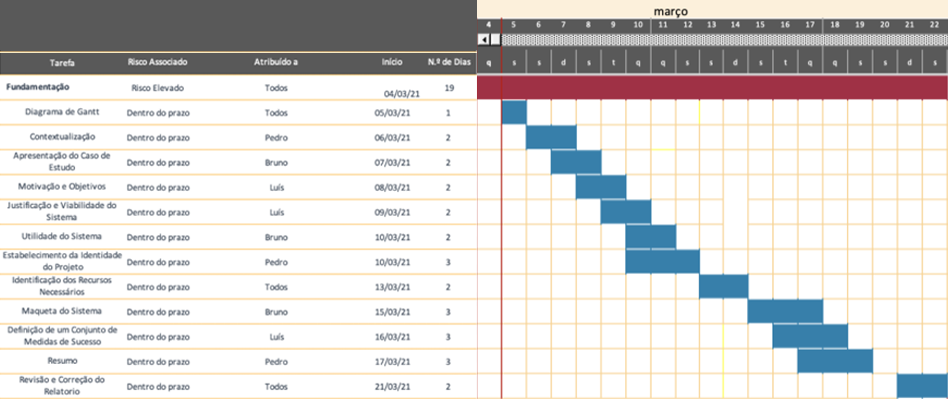
\includegraphics[width=\textwidth]{images/Fase1/plano_f1.png}}
            \caption{Plano da Fase 1}
        \end{figure}
        
        \begin{figure}[hbt!]
            \centering
            \frame{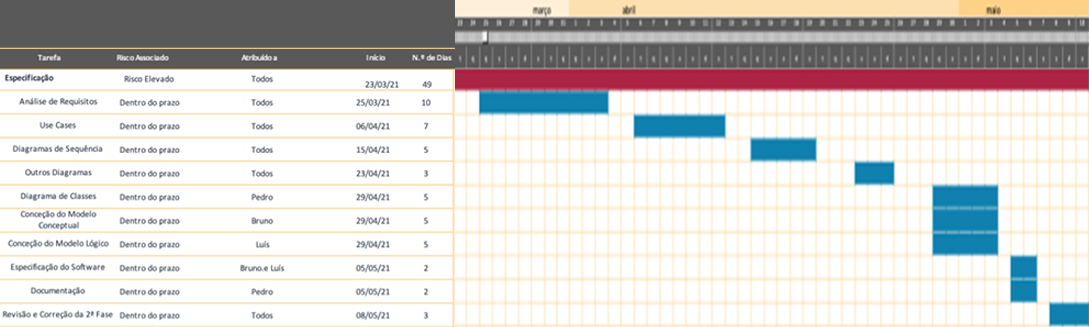
\includegraphics[width=\textwidth]{images/Fase1/plano_f2.png}}
            \caption{Plano da Fase 2}
        \end{figure}
        
        \begin{figure}[hbt!]
            \centering
            \frame{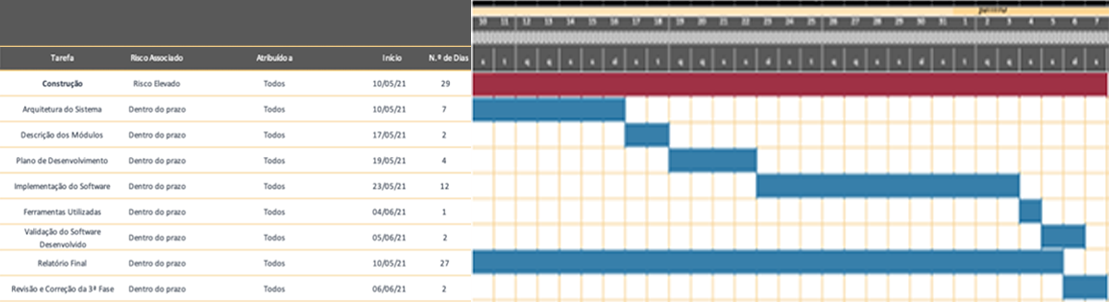
\includegraphics[width=\textwidth]{images/Fase1/plano_f3.png}}
            \caption{Plano da Fase 3}
        \end{figure}

%==========================================================================
% END INTRODUCTION
%==========================================================================


%==========================================================================
% BEGIN CONCLUSÕES E TRABALHO FUTURO
%==========================================================================

\chapter{Conclusões e Trabalho Futuro}
    \tab Terminada esta primeira fase do nosso projeto, sendo que será a mais crucial, acreditamos ter conseguido tanto criar uma base sólida para o resto do desenvolvimento do nosso sistema de monitorização como organizar todo o trabalho que ainda nos falta desenvolver.
    
    \tab Após a realização da etapa da fundamentação, a equipa conseguiu ter uma melhor perceção daquilo que é necessário fazer para concretizar a tarefa que tem em mãos e, com a observação dos diferentes Diagramas de \textit{Gantt}, a maneira como o trabalho se encontra dividido.
    
    \tab Acreditamos, assim, ter conseguido atingir todos os objetivos a que nos propusemos nesta etapa e estar prontos para avançar para a etapa da especificação, onde iremos conceber toda a modelação \textit{UML} do nosso projeto. Esperamos obter, no final de todas as etapas, uma aplicação bem conseguida, acessível a toda a população e que vá de encontro a solucionar vários problemas relacionados ao tema do nosso projeto.


%==========================================================================
% END CONCLUSÕES E TRABALHO FUTURO
%==========================================================================

%==========================================================================
% BEGIN REFERÊNCIAS
%==========================================================================

%% Changes biblibography name
%% Portuguese babel default : "Bibliografia"
%% Personally I prefer "Referências"
\renewcommand\bibname{Referências}

%% https://www.overleaf.com/learn/latex/bibliography_management_with_bibtex
\begin{thebibliography}{9}

\bibitem{incendio_pedrogao}
D. de Notícias, “Pedrógão. Chamas mataram 66 pessoas e atingiram cerca de 500 casas,” DN, 17-Jun-2019. [Online]. Available: https://www.dn.pt/pais/pedrogao-grande-chamas-mataram-66-pessoas-e-atingiram-cerca-de-500-casas-11016481.html. [Accessed: 21-Mar-2021]. 

\bibitem{relatorio_fogos_2019} 
MOREIRA, J., PEREIRA, T., CRUZ, M., 2020. Country report for Portugal in San-Miguel-Ayanz et al. (Eds), Forest Fires in Europe, Middle East and North Africa 2019, EUR 30402 EN, Publications Office of the European Union, Luxembourg, 2020, ISBN 978-92-76-23209-4, doi:10.2760/468688, JRC122115

\bibitem{corpos_bombeiros}
“Corpos de Bombeiros,” PORDATA. [Online]. Available: https://www.pordata.pt/Portugal/Corpos+de+Bombeiros-1107. [Accessed: 22-Mar-2021]. 

\end{thebibliography}


%==========================================================================
% END REFERÊNCIAS
%==========================================================================

%==========================================================================
% BEGIN LISTA DE SIGLAS E ACRÓNIMOS
%==========================================================================

%% Portuguese babel does not translate this environment
\renewcommand{\nomname}{Lista de Siglas e Acrónimos}

%% Text that can be shown before acronyms list
\renewcommand{\nompreamble}{}

%% acronyms
\nomenclature[01]{\textbf{API}}{Application Programming Interface}
\nomenclature[02]{\textbf{UML}}{Unified Modeling Language}


%% Show acronyms
\printnomenclature



%==========================================================================
% END LISTA DE SIGLAS E ACRÓNIMOS
%==========================================================================


%==========================================================================
% BEGIN ANEXOS
%==========================================================================

%% Why \addchap, instead of \chapter? 
%% \addchap has no numbering but appears in table of contents.
%\addchap{Anexos}

    %<<Os anexos deverão ser utilizados para a inclusão de informação adicional necessária para uma melhor compreensão do relatório o para complementar tópicos, secções ou assuntos abordados. Os anexos criados deverão ser numerados e possuir uma designação. Estes dados permitirão complementar o Índice geral do relatório relativamente à enumeração e apresentação dos diversos anexos.>>
    
    %% section version of \addchap
    %\addsec{Anexo 1}


%==========================================================================
% END ANEXOS
%==========================================================================
\end{document}